%%%--- Template for master thesis at SfS
%%%--- Modified template with more comments and examples -- SG, 11/06/09
%%%------
\documentclass[11pt,a4paper,twoside,openright]{report}
%%not needed \usepackage{E}
\usepackage[english]{ETHDAsfs}%--> ETHDASA + fancyheadings + ... "umlaute" 
%  + sfs-hyper -> hyperref 

\usepackage{pdfpages}%%to include the confirmation of originality (plagiarism
\usepackage{amsbsy}%% for \boldsymbol and \pmb{.}
\usepackage{amssymb}%% calls  amsfonts...
%or \usepackage{german8}%-- =  german  +  isolatin1
\usepackage{graphicx}%-- f�r PostScript-Grafiken (besser als  psfig!)
%\usepackage[draft]{graphicx} % grafics shown as boxes --> faster compilation
%
\usepackage[longnamesfirst]{natbib}%was {sfsbib}%- F�r  Literatur-Referenzen
%           ^^^^^^^^^^^^^^ 1) "Hampel, Ronchetti, ..,"  2) "Hampel et al"
% Engineers (and other funny people) want to see [1], [2] 
% ---> use 'numbers' : \usepackage[longnamesfirst,number]{natbib}
%
%
\usepackage{texab}%- 'tex Abk�rzungen' /u/sfs/tex/tex/latex/texab.sty
        %%- z.B.  \R, \Z, \Q, \Nat f�r reelle, ganze, rationale, nat�rl. Zahlen;
        %%-       \N   (Normalvert.)  \W == Wahrscheinlichkeit .....
        %%-  \med, \var, \Cov, \....
        %%-  \abs{x} == |x|   und   \norm{y} ==  || y ||   (aber anst�ndig)
%% NOTE: texab contains many useful definitions and "shortcuts". It is
%% worth to open the file and have a look at them. HOWEVER, some
%% definitions are a bit can lead to conflicts with other packages. You
%% might for example want to comment out the line defininf \IF as an
%% operator when working with the algorithmic package, or to comment out
%% the line defining a command \Cite with working with the Biblatex package  
\usepackage{amsmath}
%\usepackage{mathrsfs}% Raph Smith's Formal Script font --> provides \mathscr
\usepackage{enumerate}% Fuer selbstdefinierte Nummerierungen
%--------
\usepackage{relsize}%-> \smaller (etc) used here
\usepackage{color} %% to allow cloring in code listings
\usepackage{listings}% Fuer R-code, C-code, ....  and settings for these:
\definecolor{Mygrey}{gray}{0.75}% for linenumbers only!
\definecolor{Cgrey}{gray}{0.4}% for comments
\lstloadlanguages{R}
\lstset{ %% Hilfe unter z.B. http://en.wikibooks.org/wiki/LaTeX/Packages/Listings
language=R,
basicstyle=\ttfamily\scriptsize,%%- \small > \footnotesize > \scriptsize > \tiny
%commentstyle=\ttfamily\color{Cgrey},
commentstyle=\itshape\color{Cgrey},
numbers=left,
numberstyle=\ttfamily\color{Mygrey}\tiny,
stepnumber=1,
numbersep=5pt,
backgroundcolor=\color{white},
showspaces=false,
showstringspaces=false,
showtabs=false,
frame=single,
tabsize=2,
captionpos=b,
breaklines=true,
%breakatwhitespace=false,
keywordstyle={},
morekeywords={},
xleftmargin=4ex, 
literate={<-}{{$\leftarrow$}}1 {~}{{$\sim$}}1}
\lstset{escapeinside={(*}{*)}} % for (*\ref{ }*) inside lstlistings (Scode) 
%%----------------------------------------------------------------------------

%%------- Theoreme ---
\newtheorem{definition}{Definition}[subsection]
\newtheorem{lemma}[definition]{Lemma}
\newtheorem{theorem}[definition]{Theorem}
\newtheorem{Coro}[definition]{Corollary}
\theoremstyle{definition} 
\newtheorem{example}[definition]{Example}
\newtheorem*{note}{Note}
\newtheorem*{remark}{Remark}

\DeclareMathOperator*{\plim}{plim}
% \def\MR#1{\href{http://www.ams.org/mathscinet-getitem?mr=#1}{MR#1}}

% \newcommand{\Lecture}[3]{\marginpar{#3.#2.#1}}
% \newcommand{\Fu}{\mathcal{F}}
\newcommand{\aatop}[2]{\genfrac{}{}{0pt}{}{#1}{#2}}

%\renewcommand{\theequation}{\arabic{equation}}
\numberwithin{equation}{subsection}

%%%%%%%%%%%%%%%%%%%%%%%%%%%%%%%%%%%%%%%%%%%%%%%%%
%%% Path for your figures                      %%%
%%%%%%%%%%%%%%%%%%%%%%%%%%%%%%%%%%%%%%%%%%%%%%%%%
% Set the paths where all figures are taken from:
\graphicspath{{Pictures/}}

%%%%%%%%%%%%%%%%%%%%%%%%%%%%%%%%%%%%%%%%%%%%%%%%%
%%% Define your own commands here             %%%
%%%%%%%%%%%%%%%%%%%%%%%%%%%%%%%%%%%%%%%%%%%%%%%%%
\newcommand{\Bruch}[2]{{}^{#1}\!\!/\!_{#2}}
\renewcommand{\labelenumi}{\roman{enumi}.)}



\begin{document}
\bibliographystyle{chicago}% ---> Hampel,F., E.Ronchetti,... W.Stahel(1986) ...
 %was \bibliographystyle{sfsbib}\citationstyle{dcu} %OR DEFAULT : \citationstyle{agsm}

\pagenumbering{roman}%- roman numbering for first few pages

%%%%%%%%%%%%%%%%%%%%%%%%%%%%%%%%%%%%%%%%%%%%%%%%%
%%% Title page                                %%%
%%%%%%%%%%%%%%%%%%%%%%%%%%%%%%%%%%%%%%%%%%%%%%%%%
\period{Fall 2018}
\dasatype{Master Thesis}
\students{Christopher Salahub}
\mainreaderprefix{Adviser:}
\mainreader{Prof.\ Dr.\ Marloes Maathuis}
\alternatereaderprefix{Co-Adviser}
\alternatereader{None}
\submissiondate{March 3 2019}
\title{Seen to be done: \\ \large A statistical investigation of peremptory challenge}

\maketitle%- Titelseite wird abgeschlossen
\cleardoublepage
 %%~~~~~~~~~~~~~~~~~~~~~~~~~~~~~~~~~~~~~~~~

%%%%%%%%%%%%%%%%%%%%%%%%%%%%%%%%%%%%%%%%%%%%%%%%%
%%% Insert here acknowledgements and abstract %%%
%%%%%%%%%%%%%%%%%%%%%%%%%%%%%%%%%%%%%%%%%%%%%%%%%
%% Dedication (optional)
%\markright{}
%\vspace*{\stretch{1}}
%\begin{center}
%    To some special person
%\end{center}
%\vspace*{\stretch{2}}

% Preface (optional)
\newpage
\markboth{Preface}{Preface}
\chapter*{Preface}

I would first like to thank Prof. Dr. Marloes Maathuis for her guidance in this project, which helped me to perform my analysis
with a clear direction and purpose. In addition to the time she set aside for our bi-weekly meetings, the group meetings organized
by her Ph.D. student Marco Eigenmann were critical in the development of more nuanced analysis and intuitive visualizations
through the discussions they facilitated between me and other students. I thank Marco Eigenmann for organizing them, and Jinzhou
Li, Armin Fingerle, Sanzio Monti, and Qikun Xiang for attending my presentations and listening attentively. A special thanks is
extended to C\'edric Bleutler and Leonard Henckel, both of whom were especially engaged and participated in lengthy discussions
both during and outside of these group meetings.

I would also like to acknowledge Prof. Dr. Tilman Altwicker for his detailed literature suggestions for additional legal context
on peremptory challenges and Prof. Dr. Samuel Baumgartner for his research suggestions. Both of these provided an excellent
starting point for a first investigation of the topic. Of course, without the cooperation of Dr. Ronald Wright, Dr. George
Woodworth, Dr. Barbara O'Brien, and Dr. Catherine Grosso, all of whom generously provided me with data, the visualizations which
form the core of this work would not have been possible. As such, I am exceptionally grateful that they were so enthusiastic to
share the fruits of their labour to help cultivate mine, and hope that they find this work a fitting contribution to the
discussion of peremptory challenges.

%%% Local Variables: 
%%% mode: latex
%%% TeX-master: "MasterThesisSfS"
%%% End: 


% Abstract should not be longer than one page.
\newpage
\markboth{Abstract}{Abstract}
The legal practice of peremptory challenges is described, outlining its past and present racial controversies as well as the
modern defences typically provided in its favour. These arguments are analyzed statistically using novel visual tools including
the mobile plot and the positional boxplot, which were developed to explore the impact of race on the exercise of peremptory
challenges in three data sets (\cite{JurySunshineProj}, \cite{StubbornLegacy}, and \cite{PerempChalMurder}). Mulitnomial
regression models motivated by these visualizations are fit and used to generate precise parameter estimates which indicate the
dominance of race in peremptory challenge decisions for venire members across all data sets. Trial level summaries of the data
from \cite{JurySunshineProj} are produced and discussed in the context of the results from the venire member models.
 

%%% Local Variables: 
%%% mode: latex
%%% TeX-master: "ShortenedThesis.tex"
%%% End: 


%%%%%%%%%%%%%%%%%%%%%%%%%%%%%%%%%%%%%%%%%%%%%%%%%
%%% Table of contents and list of figures and %%%   
%%% tables (no need to change this usually)   %%%
%%%%%%%%%%%%%%%%%%%%%%%%%%%%%%%%%%%%%%%%%%%%%%%%%
\newpage
\tableofcontents
\newpage
\listoffigures
\newpage
\listoftables

%% Notations and glossary (optional)
\cleardoublepage
\phantomsection
\addcontentsline{toc}{chapter}{\protect\numberline{}{Notation}}
\markboth{Notation}{Notation}
\chapter*{Notation and Terms}
\label{c:Notation}

\section*{Terms}

In order to facilitate clarity despite brevity, a list of terms used in this paper is presented here.

\begin{description}
\item[Prosecution/State] The legal representation which presents the case for the guilt of an individual accused of breaking the law
\item[Defence] The legal reperesentation which presents the case for the innocence of an individual accused of breaking the law
\item[Acccused/Defendant] The individual accused of breaking the law
\item[Party] One of the prosecution, defence, or judge
\item[Court] All of the judge, prosecution, and defence
\item[Jury Roll] A list of individuals in a region eligible to serve on a jury, the construction of these lists varies
\item[Venire] The population sample generated using the jury roll from which a jury is selected (according to \cite{venireety}
  derived from the latin \textit{venire facias}: ``may you cause to come'')
\item[Venire Member] An individual in the venire
\item[Jury] The final group of (usually) twelve chosen venire members which judge the guilt or innocence of the
    defendant
\item[Voir dire] From old French ``to speak the truth'' (see \cite{voirety}), this is the questioning process used by the court to
  assess the suitability of a venire member to sit on the jury
\item[Challenge with Cause] An appeal by the prosecution or defence to remove a venire member from the jury selection provess due
  to a bias which is justified to the court and evaluated by the judge, an unlimited number of these challenges can be used
\item[Peremptory Challenge] The privileged removal of a venire member from the jury selection process by the prosecution or
  defence without any reason articulated, these are limited in number in the selection of a particular jury
\item[Struck] In the context of a venire member being rejected from the jury, removal by either peremptory challenge or challenge
  with cause
\item[Litigants] The accusor and the accused, in the trials with juries the accusor is almost always the government or state
\item[Disposition] The outcome of a venire member in the jury selection process: either kept, struck with cause, struck by
  prosecution, or struck by defence
\end{description}

\section*{Variables} \label{not:variables}

Across data sets and analyses, the variable names and mathematical notation will be as follows. Note that the use of a capital
letter indicates a random variable and a lowercase letter a particular realization of a random variable.

\begin{itemize}
\item $\mathbf{x}_i = (r_i,e_i,p_i,g_i,s_i)^T$: the observed explanatory variable combination for venire member $i$
\item $d \in \{1,2,3,4\}$: indicator of disposition, with the respective levels kept, struck with cause, struck by defence,
  and struck by prosecution
\item $r \in \{1,2,3\}$: indicator of venire member race, with respective levels black, other, and white
\item $e \in \{1,2,3\}$: indicator of defendant race, with levels as for the venire member race
\item $p \in \{1,2,3,4\}$: indicator of venire member political affiliation, with respective levels Democrat, Independent,
  Libertarian, and Republican
\item $g \in \{1,2\}$: indicator of venire member gender, with respective levels female and male
\item $s \in \{1,2\}$: indicator of defendant gender, with levels as for the venire member
\item $\pi_{d|jklmn} \in [0,1]$: the probability of disposition $d$ given factor levels $jklmn$, may be written as $\pi_d$ for
  convenience or given a superscript $(i)$ to indicate this probability for venire member $i$
\item $y_{djklmn} \in \mathbb{N}$: the count of venire members with $\textbf{x}_i = (d,j,k,l,m,n)^T$
\end{itemize}

This work also uses hat notation for estimates (i.e. the estimate for $\pi$ is $\hat{\pi}$ and the estimator for $\pi$ is
$\tilde{\pi}$).

%%% Local Variables: 
%%% mode: latex
%%% TeX-master: "MasterThesisSfS"
%%% End: 


\cleardoublepage
\pagenumbering{arabic}%--- switch back to standard numbering 


%%%%%%%%%%%%%%%%%%%%%%%%%%%%%%%%%%%%%%%%%%%%%%%%%
%%% Your text... Either write here directly,  %%%
%%% or even better: write in separate files   %%%
%%% that you just have to include here.       %%% 
%%%%%%%%%%%%%%%%%%%%%%%%%%%%%%%%%%%%%%%%%%%%%%%%%
\section{Introduction} \label{c:introduction}

Recent racial controversy [\cite{fiverejected}; \cite{fraughthistory}]
related to the use of the peremptory challenges in
\textit{R. v. Stanley} [\cite{GeraldStanleyVerdict}] have culminated
in the abolition of the practice in Canada by Bill C-75 [\cite{billc75}]. This leaves the jury selection process in Canada on somewhat shaky ground [\cite{trialsrisk}] and warrants a greater discussion of the practice than its use in one isolated case. A great deal of ink has
already been spilled on both sides of the debate [\cite{peremparegood}; \cite{bothwrong}; \cite{goodfirststep}], but startlingly
little of this discussion has been based on any hard, quantitive evidence on the impact of peremptory challenge in jury
selection. Unfortunately, there is a lack of relevant Canadian data, and so this paper aims to provide analysis and evidence to illuminate the topic further by considering three peremptory
challenge data sets collected in the United States: the data from \cite{JurySunshineProj}, \cite{StubbornLegacy}, and
\cite{PerempChalMurder}, henceforth the ``Sunshine,'' ``Stubborn,'' and ``Philadelphia'' data sets respectively. While this data cannot reveal anything about the alleged racial motivation of peremptory challenge use in
\textit{R. v. Stanley}, a wider view of the practice is a more sober
place to assess its role in modern jury trials than the dissection of a particular controversial case.

Of course, this work is not the first such empirical investigation. \cite{JurySunshineProj}, \cite{StubbornLegacy}, and
\cite{PerempChalMurder} have performed analysis on the factors which
impact the use of peremptory challenges in their respective data
sets. All of these
investigations indicated that race was an important factor in
determining if a venire member was struck. Numerous others have
performed unique legal, empirical, and mathematical analyses of the jury
selection process, including
\cite{hoffman1997}, \cite{vandykejurysel}, \cite{hansvidjudging}, \cite{brown1978}, and \cite{ford2010}. Most of these authors arrived at similar conclusions on the general importance of race in the exercise of peremptory challenges
and the negative impact this has on the operation and perception of justice in the jury trial system. \cite{hoffman1997} gives an
exceptionally negative analysis of peremptory challenges from a legal perspective, while the game theory analysis of
\cite{ford2010} suggests that the use of peremptory challenges may even be counter-productive.

What is, perhaps crucially, missing from this rich analysis is an effective method of communicating these results. While the
tables generated to summarize previous analyses certainly contain
all the information necessary to evaluate strike patterns, they fail
to be accessible to a casual reader, as they require commitment and sharp focus to interpret and compare. In contrast, visual
representations of the data could be used for quick
comparison and interpretation of results and would facilitate the dissemination of
empirical results of these analyses to a broader audience. This would make the work of comparing and interpreting data sets far
more intuitive than the table representations which currently dominate. This work endeavours to provide such visual tools.

Consequently, this article proceeds in four parts. Section \ref{c:background} provides the necessary legal context to understand the
motivation of the previous investigations, outlining the general jury selection procedure and modern controversies with peremptory challenges. With the necessary context provided, Section \ref{c:data} proceeds to discuss the three data sets obtained, in particular explaining the differences in data collection methods and recorded variables. Section \ref{c:analysis} provides the details and results
of the analysis performed on the different data sets. The Sunshine data serves as the centrepiece of this analysis, as it is the most comprehensive and recent of the data sets. Mobile plots are described and used to analyse the data visually, in particular to compare the Sunshine data set to the Stubborn and Philadelphia data sets. The implication of their similarities for generalization are discussed. These visual analyses motivate
model selection in \ref{sec:mods}, garnering precise estimates of the impact of race in the Sunshine data. These results and
findings are summarized in Section \ref{c:summary}. Recommendations based on the observations obtained are provided alongside suggestions for future work.

\chapter{Peremptory Challenges} \label{c:background}

As the focus of this text is the legal practice of peremptory challenges, and these are a specific practice which may not be known
in detail to the reader, a brief exploration of their history, motivation, and current use is presented here. It is not meant to
be exhaustive, but rather to provide context and references for an interested and motivated reader to learn more. Indeed, many
details have been omitted from the summary of the history here. Roughly, the presentation of the history of jury trials follows
the comprehensive and exhaustively referenced description provided by \cite{hoffman1997}, with additional context and opinion on
certain details provided by \cite{vonmosch1921}, \cite{forsythhistory}, and \cite{brown2000}. Information regarding the history of
the Canadian system was provided by \cite{brown2000} and \cite{petersen1993}.

Before reviewing the history, it is best to give some context. The central and unchanging function of a jury in a jury trial
system is to judge the innocence or guilt of an accused in light of evidence. As discussed in \cite{vonmosch1921} and
\cite{forsythhistory}, the expectation of how this act is perform has varied throughout history. In the distant past,
\cite{vonmosch1921} and \cite{hoffman1997} report that the central function of the jury was to collect evidence, and so they
assumed the role commonly performed by modern police detectives, and so the selection of the most ``trustworthy'' individuals of
some reknown was paramount. This is contrasted with the modern jury, which performs no collection of the evidence, but instead
merely judges the guilt of the accused, and is meant to be composed of a panel of peers or ``equals'' sampled at random from the
population, an idea markedly different from, but motivated by, the Magna Carta (see \cite{davismagnacar} and \cite{hoffman1997}).

Peremptory challenges are a departure from this random selection. They are a privileged removal of a venire member - to be
replaced by a new randomly selected venire member -  by either the prosecution or defence without providing a justification to the
court. The modern motivation for this was best described by Justice Byron R. White in \cite{swainvalabama}:

\begin{quote}
\centering
The function of the challenge is not only to eliminate extremes of partiality on both sides, but to assure the parties that the
jurors before whom they try the case will decide on the basis of the evidence placed before them, and not otherwise. In this way,
the peremptory satisfies the rule that, ``to perform its high function in the best way, justice must satisfy the appearance of
justice.''
\end{quote}

\section{History} \label{sec:history}

\subsection{Pre-English History}

Although precise timelines are hard to establish, there is evidence that jury trials have occurred in some form or another since
antiquity. The concept, that of judgement by a group of peers, is so ancient that it is prevalent not only in historical records,
but in myth. As \cite{hoffman1997} indicates, both Norse and Greek mythology feature groups of individuals assessing the guilt or
collecting evidence about the actions of a peer.

Outside of the realm of myth, \cite{hoffman1997} reports on evidence of the use of juries in Ancient Egypt, Mycenae, Druid
England, Greece, Rome, Viking Scandanavia, the Holy Roman Empire, and Saracen Jerusalem. It should be noted that in none of these
areas was the jury trial the primary form of conflict resolution practiced. Nonetheless, it is clear the jury trial has a broad
and long history of use.

Something similar to the modern peremptory challenge does not appear until Rome, however. The Roman \textit{Judices} were groups
of senators selected to judge the guilt of the accused in a legal case. \cite{hoffman1997} presents evidence of the selection of
81 Senators to sit on one of these \textit{Judices}, after which the litigants were permitted to remove fifteen of these Senators
each. This egalitarian reduction of the jury size seems analogous to the modern peremptory challenge system in placing the power
of removal with the litigant and suggesting no justification is necessary for their removal.

\subsection{In English Law (1066--1988)}

Peremptory challenge does not reach is modern form, with a jury size that is held constant, until it was established in the
English legal system. It should be noted that despite some previous debate on the topic, the most modern historical evidence
suggests that the basis of the English practice was not related to the system used in the selection of \textit{Judices} in
Rome. The English system appears to be its own beast entirely.

The currently accepted theory is that the jury system was introduced to England during the Norman conquest of 1066. Following
the official adoption of juries in the Assize of Clarendon in 1166, and the outlaw of trials by ordeal (the most common method of
trial at that time) in 1215, peremptory challenges began to appear in England in the late thirteenth century. The challenges were
officially recognized in 1305 when Parliament outlawed their use by the Crown, only to replace them with an analogous system of
so-called ``standing-aside''\footnote{For a detailed explanation of this system see \cite{hoffman1997}}.

It should be noted here that although the challenges issued between the Assize of Clarendon and this 1305 act are called
``peremptory,'' they may not serve the same purpose as the modern challenges. Indeed, as Hoffman argues \cite{hoffman1997}, the
challenges at this point in history may have been challenges with cause. The lack of a need to discuss the justification for such
a causal challenge can be attributed to two factors: the function of these early courts in small communities where the court would
be familiar with the venire members, and the justification of prosecution challenges under the paradigm of royal infallibility.

While the first of these, where both sides simply ``know'' why an individual is being challenged seems tenuous at best, the second
justification for the Crown's use of challenges seems quite reasonable. If the king cannot be wrong in his judgement and he has
some reason to feel that a venire member cannot serve on the jury, then it would be highly disrespectful to ask him to justify his
action. The Crown prosecutors, as representatives of the king, would be similarly shielded from criticism. The growth of
peremptory challenges from the Crown to the defence was then simply an act done out of a desire to limit the power of the monarch
and improve the chances of any individual facing royal inquiry. 

While the logic of the expansion of these challenges is lost to time, their legal limits are not. From a maximum of 35 challenges
allowed at their peak, the allowed number of challenges has only decreased over the centuries. This culminated in the Cyprus spy
case in the late 1970s, which led to a ``sustained campaign in Parliament and in the press alleging that defence counsel were
systematically abusing it.''\cite{hoffman1997} Ultimately this campaign was settled by the Criminal Justice Act of 1988, in which
the Parliament of the United Kingdom abolished the practice. It did not, however, abolish the use of ``standing-aside'' by the
Crown, although the practice has been heavily curtailed with strict guidelines to its use \cite{attgenguide}.

\subsection{In American Law (ca. 1700--1986)}

\subsection{In Canadian Law (1867--1988)}

\section{Modern Practice} \label{sec:modprac}

\subsection{In American Law}

\subsection{In Canadian Law}

\subsection{The Gerald Stanley Trial}

Whatever justification for the modern and historical practice of peremptory challenges a proponent espouses, it should be clear
from the fallout of the Gerald Stanley trial that peremptory challenges have failed in this case. Rather than guaranteeing the
creation of a mutually acceptable jury, their use inspired an atagonistic response to the verdict of the case. In the eyes of
many, justice was not done, and peremptory challenges are the specific reason cited.

While

Every time a prospective juror is peremptorily challenged we are telling that prospective juror that the foundation of this system
is not evidence, but rather rumor, innuendo, and prejudice. - Morris B. Hoffman \cite{hoffman1997}



\section{To include a picture}
\begin{figure}[hbt!]%--- Picture 'H'ere, 'B'ottom or 'T'op; '!' Try to
                    %impose your will to LaTeX
  \epsfCfile{.85}{geys-2kern} %<< no file extension
  %%         --- .85 stands for 85% of text width
  \caption[Geyser data: binned histogram, Silverman's and another
  kernel]%<<-- Legend for the list of figures at the beginning of you thesis
  {Old Faithful Geyser eruption lengths, $n=272$; binned data and two
    (Gaussian) kernel density estimates ($\times 10$) with $h=h^*= .3348$
    and $h= .1$ (dotted).}% legend displayed below the graph.
  \label{fig:geys1}
\end{figure}

Or also with \texttt{includegraphics}:
\begin{figure}[hbt!]%--- Picture 'H'ere, 'B'ottom or 'T'op; '!' Try to
                    %impose your will to LaTeX
  \centering
  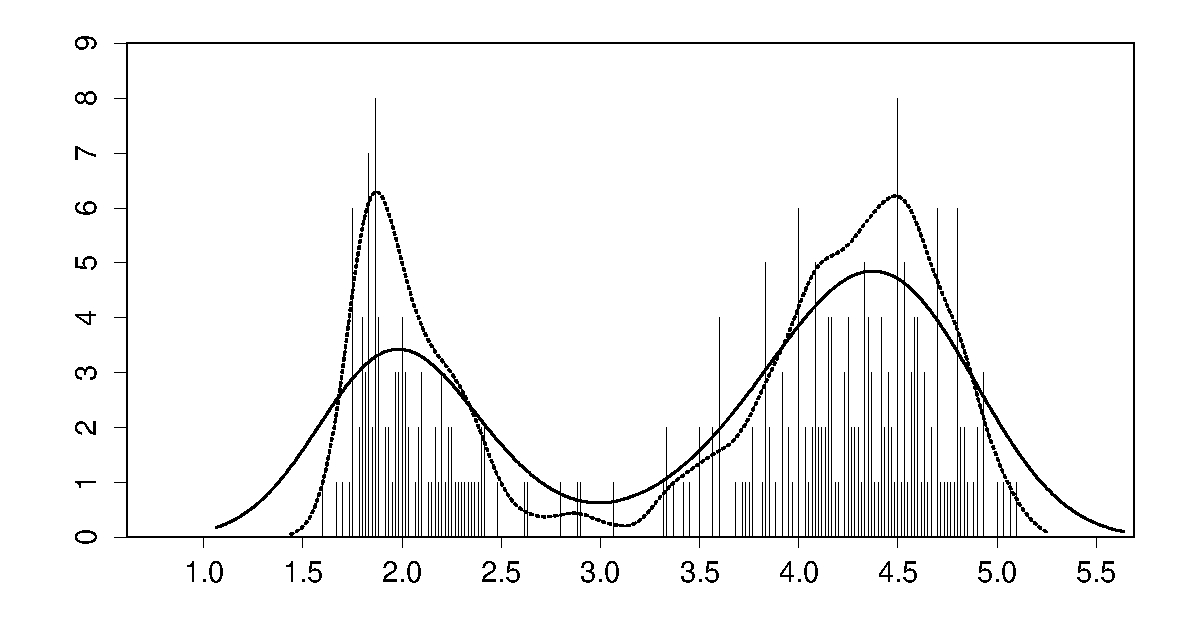
\includegraphics[width=.5\textwidth]{geys-2kern} %<< no file extension
  %%         --- .5\textwidth stands for 50% of text width
  \caption[Geyser data: binned histogram, Silverman's and another
  kernel]%<<-- Legend for the list of figures at the beginning of you thesis
  {Old Faithful Geyser eruption lengths, $n=272$; binned data and two
    (Gaussian) kernel density estimates ($\times 10$) with $h=h^*= .3348$
    and $h= .1$ (dotted).}% legend displayed below the graph.
  \label{fig:geys2}
\end{figure}

\section{To make a proof}
\begin{proof}
  $1 + 1 = 2$
\end{proof}

\section{To include \Rp code}
See information in Appendix~\ref{app:complement}.


\section{Other information}
Put a text between quotes: make sure to use nice quotes, such as ``quote''.

Cite a document in the bibliography (an example here): \cite{Reference}.
%%--> in file   myReferences.bib  (same directory)
Or mention that \citeauthor{HamF85} (a person) or \citeauthor{StaWW91} (two
persons) have already done quite a bit work.

Referencing a different part of your work: please refer to Appendix \ref{app:complement}.


%%% Local Variables: 
%%% mode: latex
%%% TeX-master: "MasterThesisSfS"
%%% End: 

%%\include{Chapter...}
\section{Summary}
\label{c:summary}

The visual tools and models presented here support the dominant analysis in the literature. The primary determinant in the
exercise of peremptory challenges is race in the Sunshine data set. The prosecution tends to remove more racial minority venire
members than expected and fewer white venire members than expected. The defence tends to have the
opposite strategy. This pattern is not only seen in aggregate in \ref{sec:impactrace}, but is visible in the trial summaries
presented in \ref{sec:casesum}. The impact of race remains apparent in the mobile plots even when other legitimate factors
such as political affiliation are controlled.

Beyond detecting the patterns in one data set, this work demonstrates other strengths of the mobile plot and visual
analysis. The first of these is the utility of the mobile plot to compare the strike patterns across multiple data sets. The
similarities between the Stubborn, Philadelphia, and Sunshine data sets are immediately clear when visualized appropriately. This
is critical in examining the practice of peremptory challenges, as it allows for a comparison of their use across studies with
radically different study populations so long as analogous data is collected.

In this case, the strength of the similarities observed between these data sets when visualized with the mobile plot suggests the
pattern of racial preferences is not a local phenomenon in location or time, but is a reflection of a strategy utilized by the
prosecution and defence in jury trials generally. As more data and investigation take place, further visual comparisons can
motivate more analysis of the similarities between these patterns in different studies. Based on the findings here and in the
other empirical analyses, the critical data which should be collected for analysis is the disposition of the venire members and
the demographic characteristics of both the venire member and
defendant. Attitudinal data, which was not standardized in the data
analysed in this work, should also be collected and analyzed in some standard way to augment the utility of the mobile plot for comparison.

Another strength of the mobile plot is the motivation of model building. The multinomial regression models from \ref{sec:mods}
were created to fit models analogous to the displayed patterns of the mobile plots generated in advance. That the findings of the
models matched the analysis of the mobile plots almost exactly justifies these plots as informative analytical tools. The models
allowed for the estimation of effects in the Sunshine data controlling for possible legitimate confounders, giving a table of
coefficient estimates consistent with those generated previously for other data sets, such as the Stubborn and Philadelphia data.

It was not until these coefficients were visualized with the dot-whisker plot, however, that a number of more nuanced patterns
became obvious. The first of these is the greater sensitivity of the
defence to the racial aspects of a trial than the
prosecution. That is, the race of the venire member has a greater impact on the defence's probability of rejection than the
prosecution's. The second pattern is the tendency of race matching by
the defence and race contrasting by the prosecution. This aggregate pattern also seems to be reflected in the trial level
summary of the data, which suggests that this trend is not a quirk of
aggregation, but a reflection of individual lawyer decision making.

Of course, as suggestive as these patterns are, and as spotted as the history of peremptory challenges is with controversy, none
of this can say definitively whether the individuals rejected from the
Sunshine venires were rejected appropriately due to their ``extreme''
bias. Without detailed descriptions of the bias of the population as a whole, such judgements on the propriety of strikes simply
cannot be made, and whether these racial strike patterns are simply the result of legitimate strikes issued for reasons related
strongly to race remains unknown.

Despite this limitation, the final scatterplots suggest a criticism of
peremptory challenges independent of these concerns which is consistent with the source
of controversy for \textit{Batson v. Kentucky}, \textit{Swain v. Alabama}, and \textit{R. v. Stanley}. Peremptory challenges
frequently remove all representatives of minority groups from the
venire. This prevents their participation in a panel meant to
represent the conscience of their community, corroding a critical function of the jury and creating a group
sceptical of the operation of the legal system. Certainly, the smaller sizes of minority groups and their relationship to the
majority may lead to their under-representation for reasons other than peremptory challenges, but a graphical exploration shows
definitively that a component of their under-representation is
peremptory challenges. Minority groups are fully struck from the
venire by peremptories far more often than majority groups. Striking
all majority members may, in fact, be virtually impossible.

All of this paints a bleak picture of the role of peremptory challenges in the modern jury selection process. Without additional
work, it is impossible to say with certainty whether the racial patterns observed here and elsewhere are due to racial prejudice
by the court, but one may ask the question of whether that matters. As Lord Chief Justice Hewart said in \textit{R. v. Sussex
  Justices}

\begin{quote}
  Justice should not only be done, but should manifestly and undoubtedly be seen to be done
\end{quote}

The visualizations of this paper have made much seen, but it is doubtful that what has been seen here, and by the critics of the
\textit{R. v. Stanley} proceedings, looks like justice.

\section{Future Work}
\label{sec:FutureWork}

One obvious way to extend the work done here is through more thorough modelling. While the multinomial regression model fit in
\ref{sec:mods} served its purpose, much more precise models could be fit using causal graphs. Such causal modelling has the
possibility to extend the observations of the model from the simple pattern identification of the multinomial model and
visualizations presented here to precise statements about the magnitude of causal effects between factors. Representing the
factors in a causal graph would also be a useful exercise in making the assumptions of the model abundantly clear. Logistic
regression models and multinomial models, which have been the norm for peremptory challenge data so far, are less clear about
their assumptions, especially to those not trained to fit and analyse these models.

Other possible models of interest are mixed models. In this work the attempts to fit mixed models were not discussed, but at
several points models with random effects for each trial were attempted. Unfortunately, these models failed to converge. Not a
great deal of time was spent trying to transform the data to facilitate convergence to a reasonable value, and so no mixed models
were fit. Such models are attractive because they have the potential to flexibly control for a host of factors which will vary
between trials, and do so in a manner which involves minimal parameters. Estimating a random effect for lawyer,
for instance, could shed light on how variable lawyers are in their behaviour. This dimension of individual variability is
essentially unadressed by the aggregate examinations of this work.

Another extension would be further investigation of the Sunshine data. It is an incredibly rich data set and this work only
examined one small facet of it. The crime classification outlined in \ref{sec:jspdata}, for example, was never utilized in the
analysis, despite the investment of time and effort in performing this clean up. Perhaps this method could also be
applied to other irregular data in court cases or elsewhere to efficiently categorize irregular strings.

Finally, as \cite{JurySunshineProj} notes, more data is needed on this topic generally. Further efforts to collect data and
reinforce or refute the findings of this work and previous ones should be undertaken, and efforts to centralize and regularize the
data would assist in the ease of analysis. Using the visualizations of
this paper, such as the mobile plot and positional boxplot, quick and
informative comparisons of new data to older data sets could be
performed easily. Increased transparency and
centralized data collection additionally have the potential to allow for a greater understanding of which elements of the jury
trial system work and which are inappropriate. As \citeauthor{JurySunshineProj} puts it:

\begin{quote}
  The transformative power of data ... could improve the courts' efforts to regulate the work of other
  criminal justice players, such as police and prosecutors.
\end{quote}

%%% Local Variables: 
%%% mode: latex
%%% TeX-master: "MasterThesisSfS"
%%% End: 
 

%%%%%%%%%%%%%%%%%%%%%%%%%%%%%%%%%%%%%%%%%%%%%%%%%
%%% Bibliography                              %%%
%%%%%%%%%%%%%%%%%%%%%%%%%%%%%%%%%%%%%%%%%%%%%%%%%
\addtocontents{toc}{\vspace{.5\baselineskip}}
\cleardoublepage
\phantomsection
\addcontentsline{toc}{chapter}{\protect\numberline{}{Bibliography}}
\bibliography{myReferences}
%% All books from our library (SfS) are already in a BiBTeX file
%% (Assbib). You can use Assbib combined with your personal BiBTeX file:
%% \bibliography{Myreferences,Assbib}. Of course, this will only work on
%% the computers at SfS, unless you copy the Assbib file 
%%  --> /u/sfs/bib/Assbib.bib

%%%%%%%%%%%%%%%%%%%%%%%%%%%%%%%%%%%%%%%%%%%%%%%%% 
%%% Appendices (if needed)                    %%%
%%%%%%%%%%%%%%%%%%%%%%%%%%%%%%%%%%%%%%%%%%%%%%%%%
\addtocontents{toc}{\vspace{.5\baselineskip}}
\appendix
\chapter{Complementary information}
\label{app:complement}

Additional material. For example long mathematical derivations could be
given in the appendix. Or you could include part of your code that is
needed in printed form. You can add several Appendices to your thesis (as
you can include several chapters in the main part of your work).

\section{Including \Rp code with verbatim}
A simple (rather too simple, see~\ref{App:listings}) way to include code or
{\it R} output is to use 
\texttt{verbatim}. It just prints the text however it is (including all
spaces, ``strange'' symbols,...) in a slightly different font.
\begin{verbatim}
## loading packages
library(RBGL)
library(Rgraphviz)
library(boot)

## global variables
X_MAX <- 150

   This allows me to put as many s  p a   c es   as I want.
I can also use \ and ` and & and all the rest that is usually only 
accepted in the math mode.

I can also make as 
                  many 
             line 
    breaks as 
I want... and
             where I want. 
\end{verbatim}

\section{Data Processing Code}\label{app:proccode}
However, it is much nicer to use the \emph{listings} package to include \Rp
code in your report. It allows you to number the lines, color the comments
differently than the code, and so on.

\lstinputlisting{Pictures/DataProcess.R}


\section{Jury Sunshine Irregularities} \label{app:irregs}

\begin{table}[h]
  \caption[Jury Sunshine Irregularities]{Jury sunshine data irregularities noted in data flattening}
  \centering
  \begin{tabularx}{\textwidth}{|c|X|} \hline
    Charges without trial (ACISID) & 08CRS50940, 08CRS52888, 09CRS000305, 09CRS1106, 09CRS50752, 10CR52031, 10CRS051975,
    10CRS1215, 10CRS397, 10CRS51388, 10CRS51610, 10CRS52410, 11CRS051642, 11CRS051795, 11CRS1577, 11CRS1745, 11CRS1783,
    11CRS51204, 11CRS51895, 11CRS52470, 08CRS54836, 08CRS50113 \\ \hline 
    Prosecutors without trials (IDs) & 1-000, 11B-000, 12-000, 14-000, 15B-000, 16A-000,
                     16B-000, 17A-000, 17B-000, 19A-000, 19B-000,
                     20A-000, 20B-000, 21-000, 22A-000, 22B-000,
                     24-000, 25-000, 27A-000, 27B-000, 28-000,
                                       29A-000, 29B-000, 30-000, 6-000, 9-000 \\ \hline
    Trial missing charge (ID) & 710-01 \\ \hline
  \end{tabularx}
\end{table}

\section{Jury Sunshine Charge Classification} \label{app:charge}

\begin{figure}[!h]
  \centering
  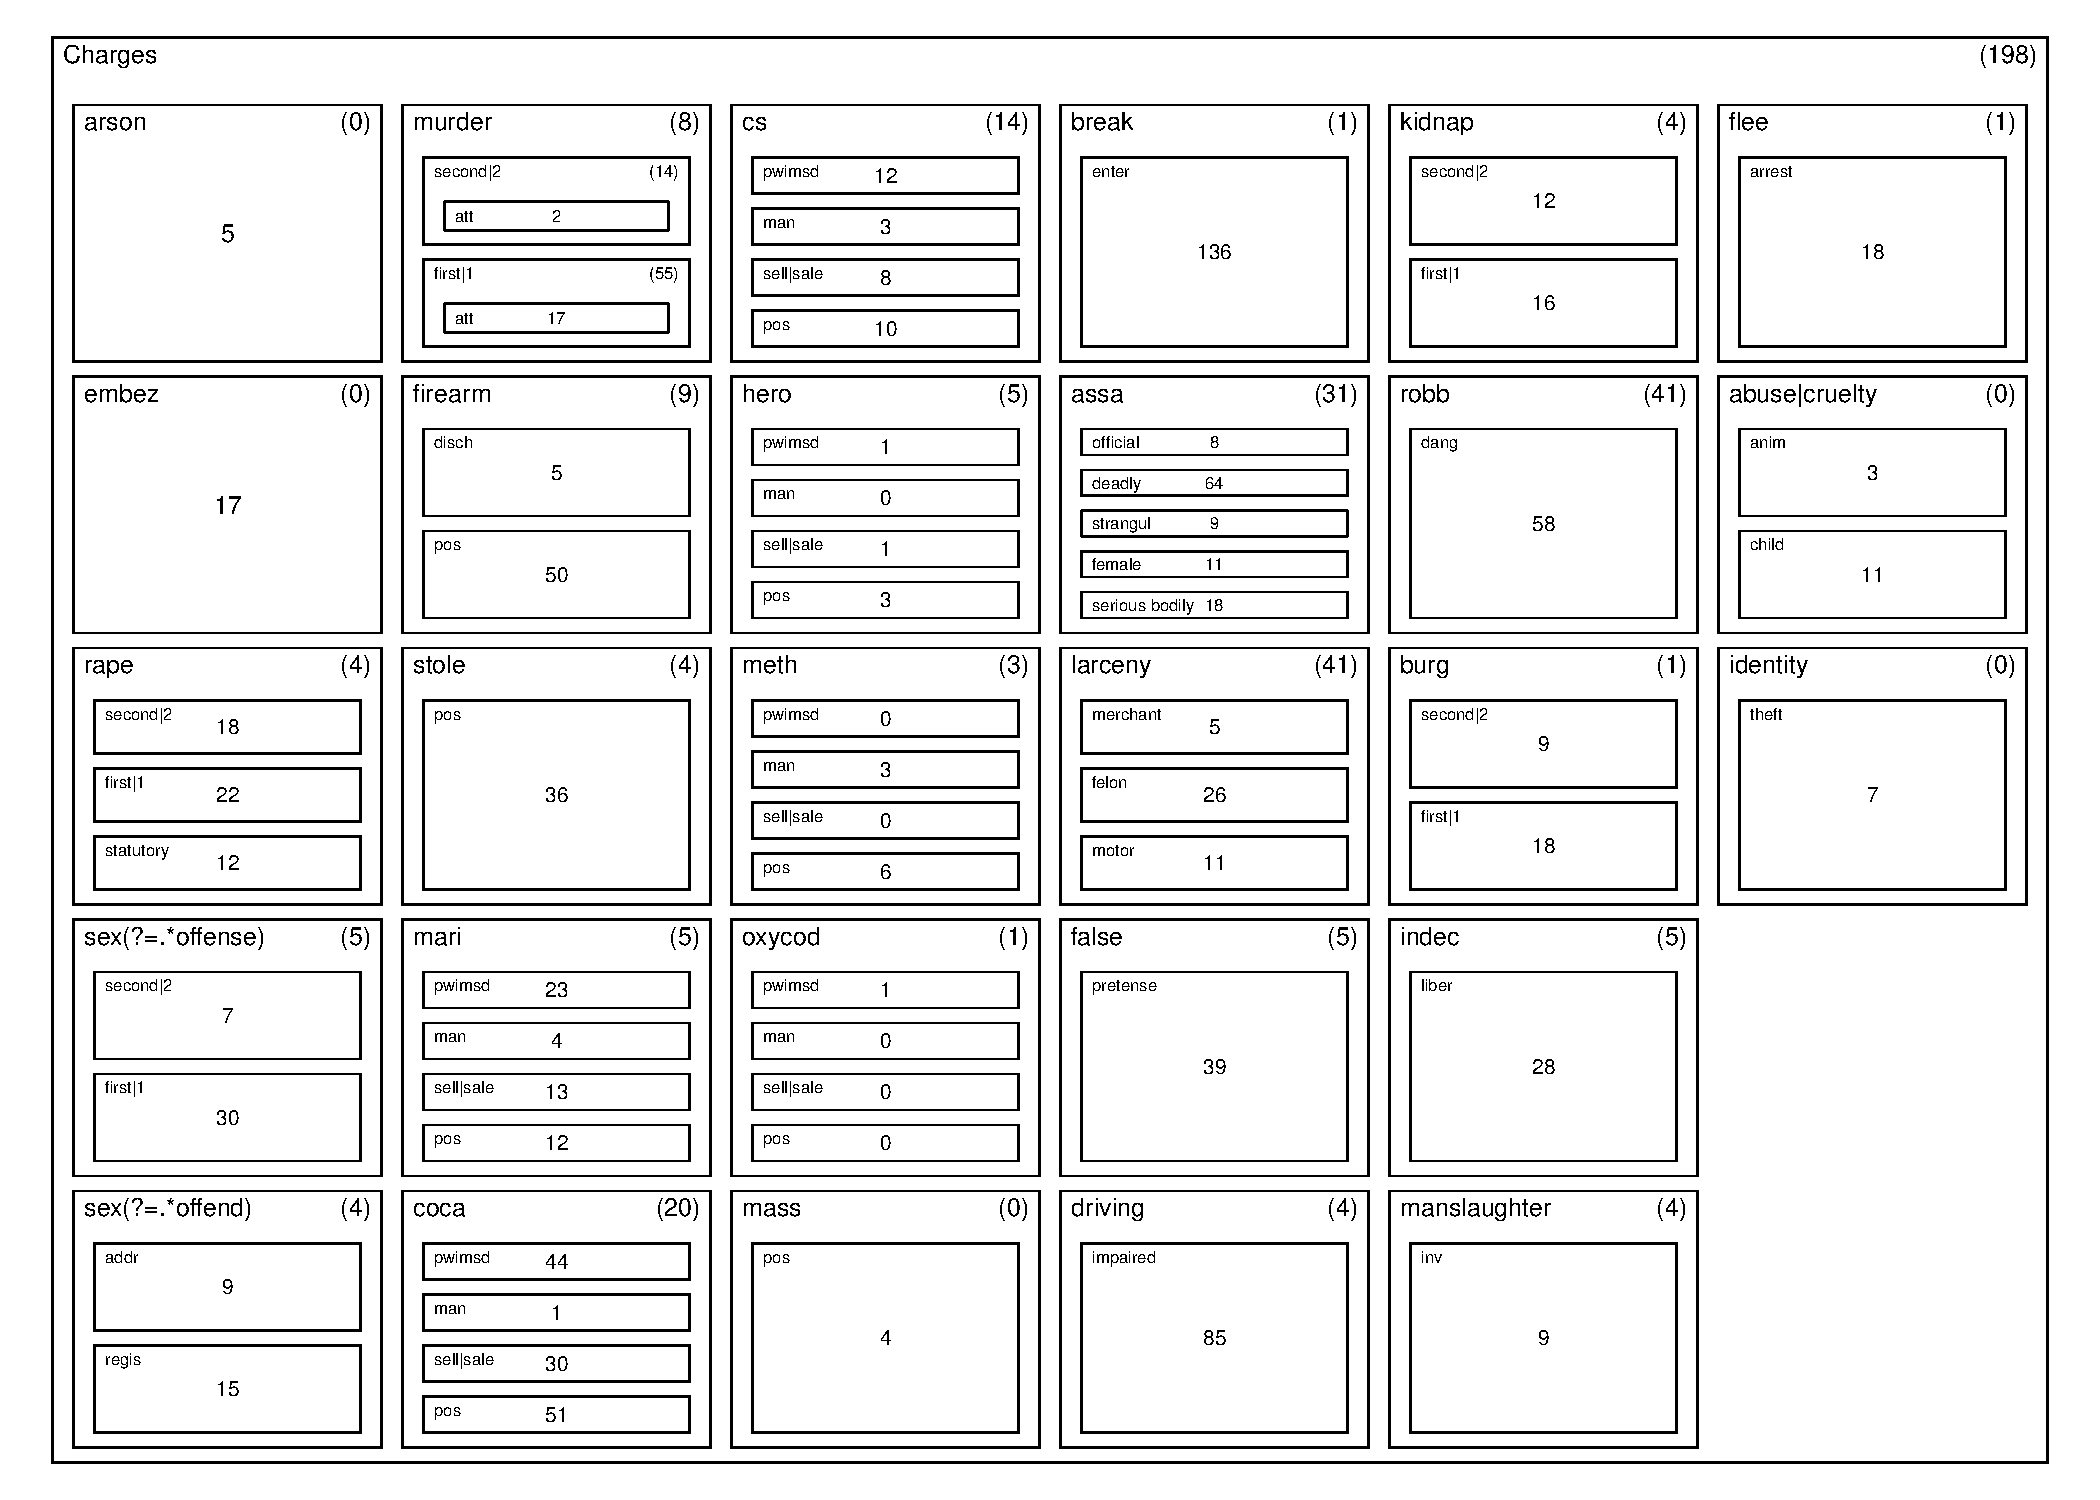
\includegraphics[angle=90, origin=c, width=1\textwidth]{ChargeDiagram}
  \caption[Regular expression charge tree visualized]{The regular expression charge tree arranged by hierarchy with counts
    provided. The counts in brackets indicate the counts of charges which could not be classified to a lower level of the
    hierarchy}
  \label{fig:chargetree}
\end{figure}

\section{Analysis Code} \label{app:analysis}

\lstinputlisting{Pictures/AnalysisScript.R}

\section{Using Sweave to include \Rp code (and more) in your report}
The easiest (and most elegant) way to include \Rp code and its output (and
have all your figures up to date with your report) is to use Sweave. You
can find an introduction Sweave in \texttt{/u/sfs/StatSoftDoc/Sweave/Sweave-tutorial.pdf}.

%%% Local Variables: 
%%% mode: latex
%%% TeX-master: "MasterThesisSfS"
%%% End: 

\chapter{Yet another appendix....}

\section{Description}
\begin{description}
\item[Something] details.
\item[Something else] other definition.
\end{description}

\section{Tables}
Refer to Table~\ref{tab:example} to see a left justified table with caption
on top.

\begin{table}[ht]
\centering
\caption[Test results]{\label{tab:example}Results.}
\begin{tabular}{ll}
\hline
\textbf{Student} & \textbf{Grade}\\
\hline
Marie  & $6$\\
Alain  & $5.5$\\
Josette  & $4.5$\\
Pierre  & $5$\\
\hline
\end{tabular}
\end{table}

%%% Local Variables: 
%%% mode: latex
%%% TeX-master: "MasterThesisSfS"
%%% End: 



%% Epilogue (optional)
\addtocontents{toc}{\vspace{.5\baselineskip}}
\cleardoublepage
\phantomsection
\addcontentsline{toc}{chapter}{\protect\numberline{}{Epilogue}}
\markboth{Epilogue}{Epilogue}
\chapter*{Epilogue}
\label{s:Epilogue}

I came into this project broadly sceptical of the attempt to change the legal system by the removal of peremptory challenges,
fully expecting a thorough analysis to justify my distaste at the politics of the response to the verdict of
\textit{R. v. Stanley}. It is easy for a government to take action which appears good for political points before considering the
consequences. After reading the history of peremptory challenges, studying legal analyses of the practice, and viewing data for
myself, however, I am convinced that the abolition of the practice may be the best path forward. \cite{hoffman1997} was perhaps
the best argument I saw from either side of the debate, and \citeauthor{hoffman1997}'s full-throated support of the complete
abolition of peremptory challenges was incredibly influential in developing this view.

That said, as a statistician, I cannot allow myself to say that the empirical analysis in this paper proves anything. As is
generally the case with social data, there are so many possible confounders and conflicting factors that it would be easy to
mistake a pattern for something it is not. Regardless, my hope is that the visualizations presented are considered useful in the
continued investigation of this social phenomenon and others. While the solution may not be clear yet, I believe these displays
are useful visual tools to help arrive at the solution.



%%% Local Variables: 
%%% mode: latex
%%% TeX-master: "MasterThesisSfS"
%%% End: 



%%%%%%%%%%%%%%%%%%%%%%%%%%%%%%%%%%%%%%%%%%%%%%%%%% 
%%% Declaration of originality (Do not remove!)%%%
%%%%%%%%%%%%%%%%%%%%%%%%%%%%%%%%%%%%%%%%%%%%%%%%%%
%% Instructions:
%% -------------
%% fill in the empty document confirmation-originality.pdf electronically
%% print it out and sign it
%% scan it in again and save the scan in this directory with name
%% confirmation-originality-scan.pdf 
%%
%% General info on plagiarism:
%% https://www.ethz.ch/students/en/studies/performance-assessments/plagiarism.html 
\cleardoublepage
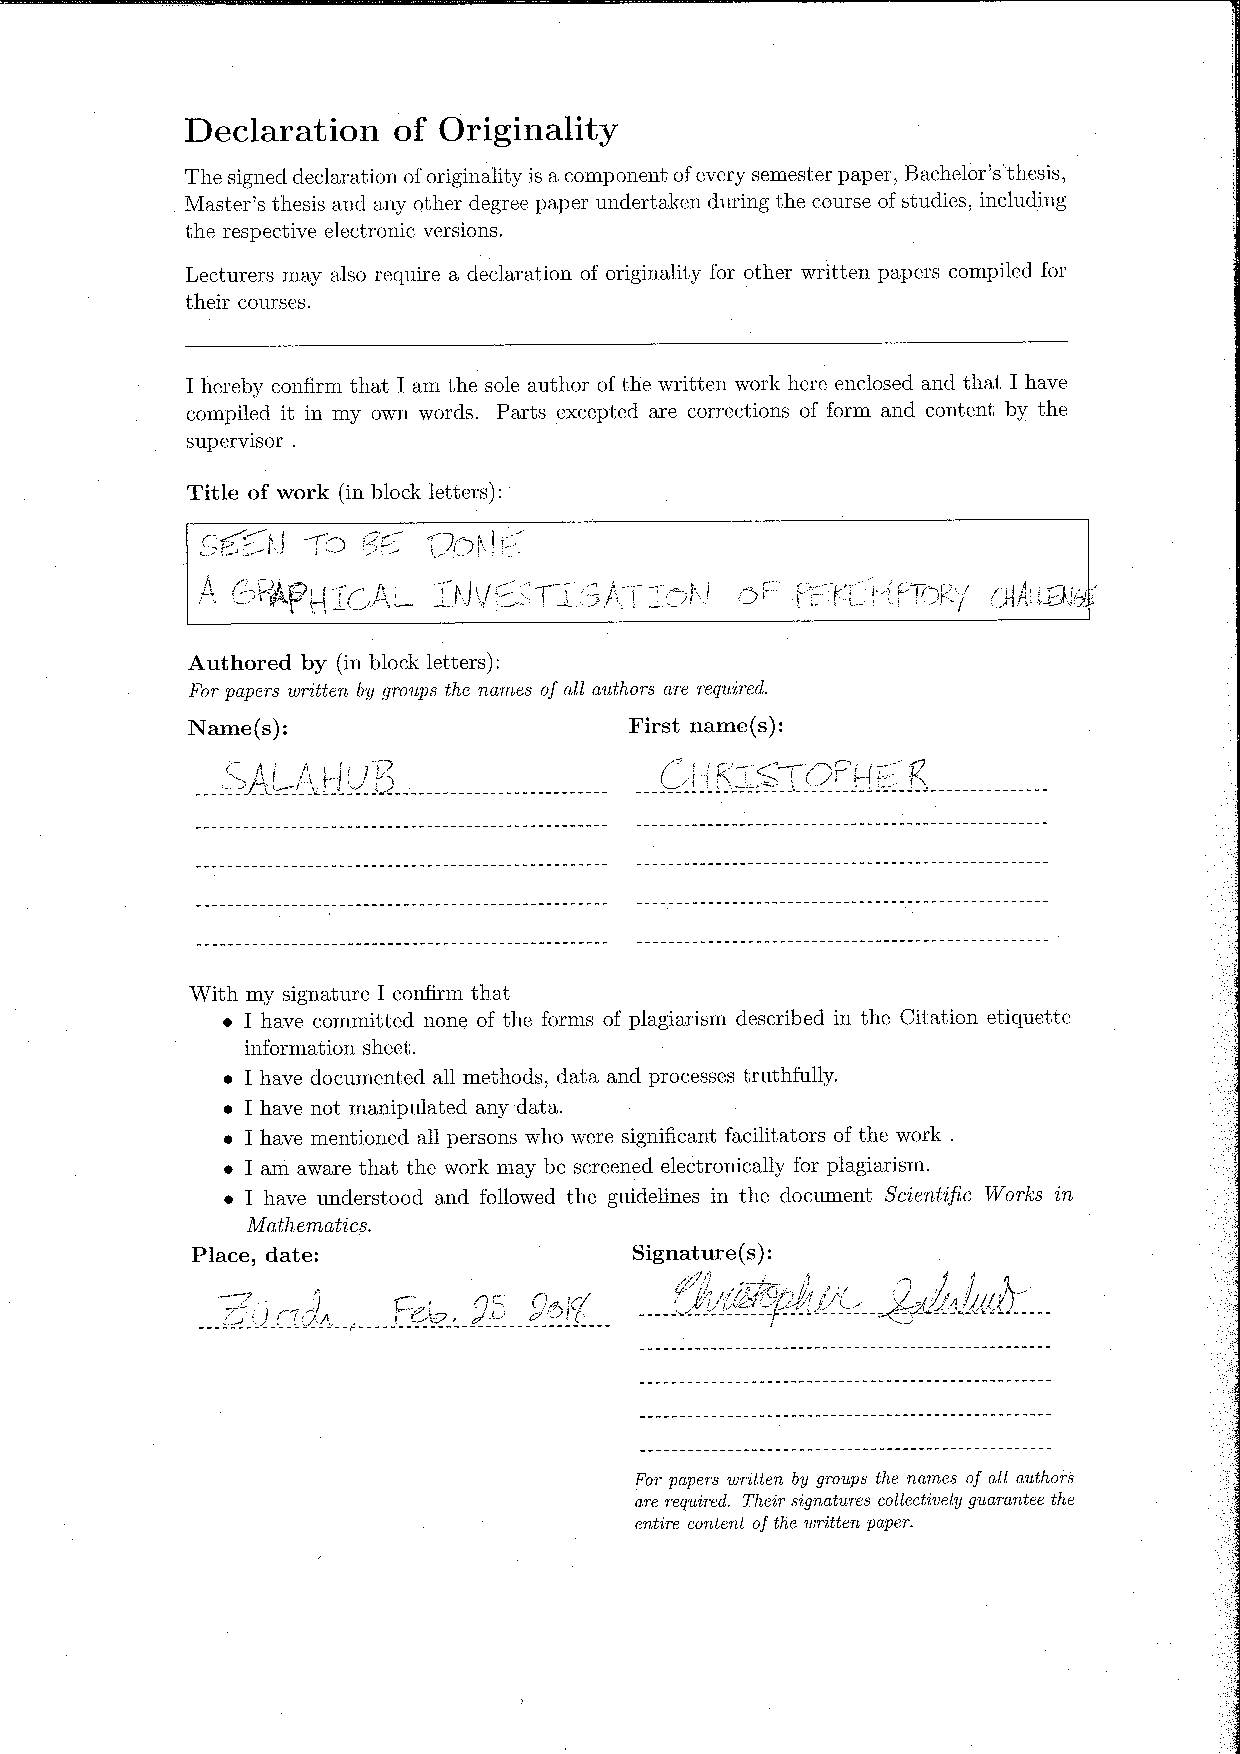
\includepdf[pages={-}, frame=true,scale=1]{confirmation-originality-scan.pdf}
\end{document}
